\documentclass[12pt]{article}
% Margin fixes
\oddsidemargin -0.5in
\evensidemargin -0.5in
\textwidth 7.25in
\topmargin 0.0in

\headheight 0.0pt
\headsep 0.0pt
\voffset 0.0pt
\textheight = 9.0in
\usepackage{amsmath,amssymb,graphicx,float}

\title{Two Slit Interference}
\author{Nathan Grouse\\Lisa Tran}

\newcommand{\counts}{\text{ counts}}

% Start the document!
\newcommand{\documentname}{\textsl{Article}}
\begin{document}
\maketitle

\section{Introduction}
\indent \indent To perform a very precise two slit interference experiment by the use of micrometer screws. We were also meant to form a low intensity experiment with an incandescent light bulb, but there was not enough time to even start this portion of the experiment.

\subsection{Apparatus}
\indent \indent The apparatus included micrometer screws, an incandescent bulb, a laser diode, a photodiode detector, and a PMT for the low intensity bulb. There were three slits corresponding to the two slit half of the experiment. First the laser passed through a single slit, then a double slit, then a blocker slit. The blocker slit could be adjusted to block one of the double slits.

\begin{figure}[H]
\centering
\hspace{-0.0in}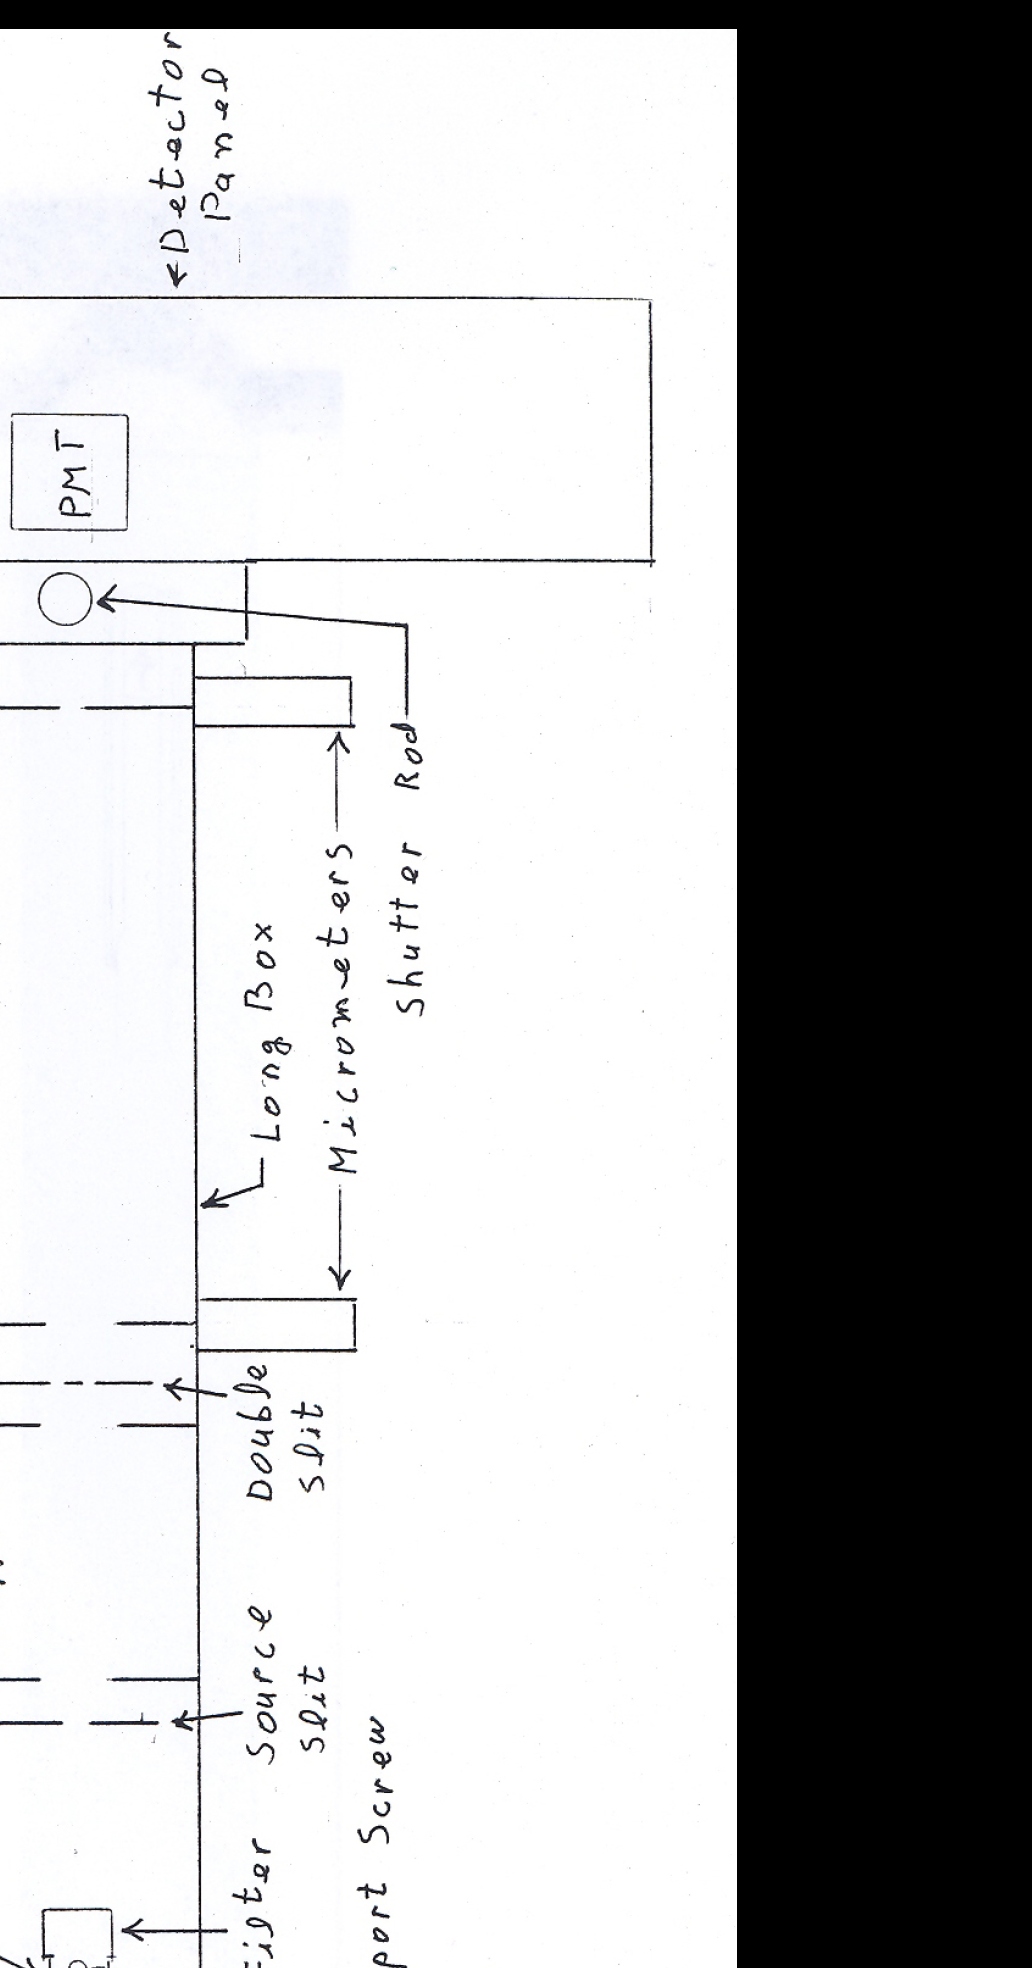
\includegraphics[scale=0.40]{apparatus.png}
\caption{Apparatus \label{fig:setup}}
\end{figure}

\section{Theory}
\indent \indent This equation is mentioned but not dervied:
\[ I = I_0 cos^2[\pi d sin \theta](\frac{sin[\pi a sin\theta / \lambda]}{\pi a sin\theta / \lambda})^2 , \]
\indent \indent where $I_0$ is the intensity in the forward direction ($\theta$ = 0) and $\lambda$ is the wavelength of the light. I don't know of any simple argument for finding the maxima of intensity for a diffraction pattern. It's possible to derive it using the Fraunhofer diffraction integral.

\section{Data}

\begin{figure}[H]
\centering
\hspace{-0.0in}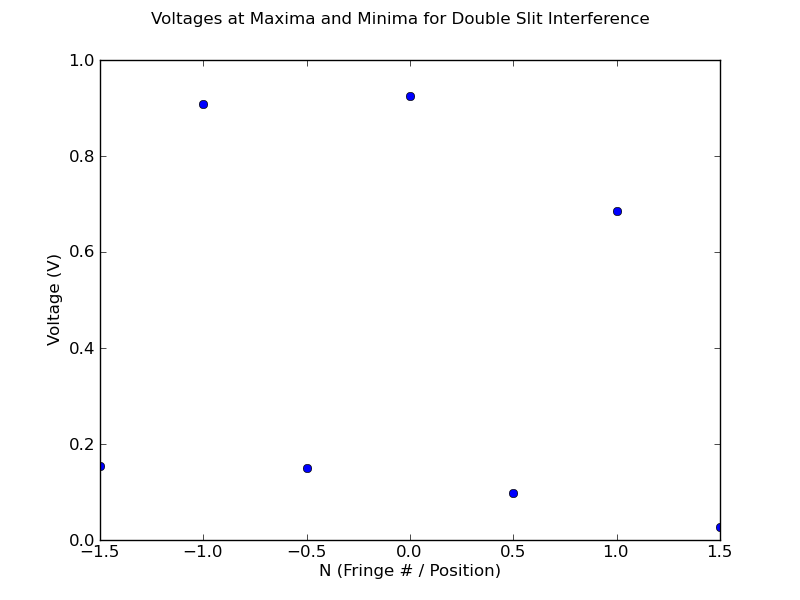
\includegraphics[scale=0.60]{Plot1.png}
\caption{Integer values of N correspond to maxima, while fractional values correspond with minima. \label{fig:setup}}
\end{figure}


\section{Calculations}
\indent \indent Ratio of the maximum intensity for two slit pattern to the maximum for the one slit pattern:
\[ \frac{I_d}{I_s} = \frac {.935 V}{.382 V} = 2.448 \]
\indent \indent Before the light reaches the two slits, it is diffracted by a single slit, so when one of the double slits is covered only about half of the diffracted light will make it to the photodiode detector. \\

\indent \indent The separation between the two slits would be given by the difference in micrometer position when each respective slit is covered:
\[ \Delta S = S_1 - S_2 = 4.50 mm - 2.80 mm = 1.70 mm \]
\indent \indent This seems larger than the separation should be, but our other readings also indicate that the slit separation is about 2 mm. The reading is accurate but not neccesarily precise.

\section{Error Analysis}
\indent \indent There was uncertainty in the voltage and micrometer readings. The voltage readings were accurate out to three decimal places, so the uncertainty in these readings is $\pm$.0005 V. The distance represented between two ticks on the micrometer is given by $\frac{.5 mm}{50 ticks} = \frac{x mm}{1 tick}$. The result is .01 mm, or 10 microns. The uncertainty in these readings is $\pm$.005 mm or $\pm$ 5 microns. //

\indent \indent Backround noise in voltage readings was recorded: .009 V. This value was used to make the data plots.
\section{Conclusion}
\indent \indent I obtained reasonable results and I saw what I expected to see. Unforuntately, I was not able to complete the entire experiment.  Had I done that half of the experiment, I would have calibrated the light bulb and detecting equipment, and allowed light to pass through both slits. Next, because the pulses are random, I would have recorded the number of counts in ten short intervals and averaged those counts to find the standard deviation $\sigma$. I would have followed the lab manual. The questions to this section are not answerable without data from this section.


\section{Questions}
\indent \indent 1. Is light a wave or a particle? \\
Ask Feynman. \\

2. How is it possible that an interference pattern is produced when there is at best only one photon in the apparatus at one time? \\
Definitely ask Feynman. \\

3. For what values of $\theta$ is the intensity I zero? \\
\[ $\pi d sin \theta / \lambda = n\frac{\pi}{2}$, where n is any odd integer \]
\[ $\pi a sin \theta / \lambda = n\pi$ where n is zero or any integer\]
\indent \indent Isolating $\theta$ in either or those expressions will give all values for $\theta$ where intensity is zero. \\

4. You should find the position of the detector slit for which the intensity of the two slit pattern is less than that for the one slit pattern. As less light is beig transmitted in the latter case, how do you explain this? \\
The nature of diffraction is that the intensity decreases as the maxima are further from the central maximum. \\



\end{document}